%% Appendix-Portfolio.tex
%% Mac Radigan
%
%% Portfolio summary results from from Markowitz-C++ Example

\section{Appendix A: The Example Portfolio}
\label{sec:appendix_a}

\subsection{Portfolio \#1: AAPL, JPM, LMT, XOM}

\newline

\begin{table}[!ht]
\begin{center}
\begin{tabular}{ l l l l }
\toprule
\multicolumn{5}{ c }{ \textbf{Portfolio \#1 (AAPL, JPM, LMT, XOM)} } \\
\hline
\textbf{Symbol} & \textbf{Weight} & \textbf{ROI} & \textbf{Volatilty} \\ \hline
AAPL   & 0.08 & 11.4\% & 28.8\% \\
JPM    & 0.12 & 31.6\% & 19.1\% \\
LMT    & 0.39 & 55.8\% & 16.3\% \\
XOM    & 0.40 & 08.2\% & 13.0\% \\ 
\hline
portfolio & &  25.0\% & 11.76\% \\ 
\hline
\bottomrule
\end{tabular}
\caption{Portfolio \#1}
\end{center}
\end{table}

\newline

\begin{figure}[H]
\begin{center}
\resizebox{7in}{!}{\includegraphics{results/portfolios/AAPL_JPM_LMT_XOM/Portfolio.eps}}
%\includegraphics{results/AAPL_JPM_LMT_XOM/Portfolio.eps}
\end{center}
\caption{Portfolio Performance}
\label{fig:portfolio_aapl_jnj_lmt_xom}
\end{figure}


%% *EOF*
